\documentclass{article}%
\usepackage[T1]{fontenc}%
\usepackage[utf8]{inputenc}%
\usepackage{lmodern}%
\usepackage{textcomp}%
\usepackage{lastpage}%
\usepackage[head=40pt,margin=0.5in,bottom=0.6in]{geometry}%
\usepackage{graphicx}%
%
\title{\textbf{Vecchio: Tratar de detener a Guaidó aceleraría la salida del dictador}}%
\author{EL NACIONAL}%
\date{04/03/2019}%
%
\begin{document}%
\normalsize%
\maketitle%
\textbf{URL: }%
http://www.el{-}nacional.com/noticias/vecchio{-}tratar{-}detener{-}guaido{-}aceleraria{-}salida{-}del{-}dictador\_273307\newline%
%
\textbf{Periodico: }%
EN, %
ID: %
273307, %
Seccion: %
EE UU\newline%
%
\textbf{Palabras Claves: }%
Estados Unidos, Carlos Vecchio\newline%
%
\textbf{Derecho: }%
2.1%
, Otros Derechos: %
\newline%
%
\textbf{\textit{El embajador de Venezuela ante Estados Unidos aseguró que~la detención de Guadió significaría el error más grande que pudieran cometer los oficialistas}}%
\newline%
\newline%
%
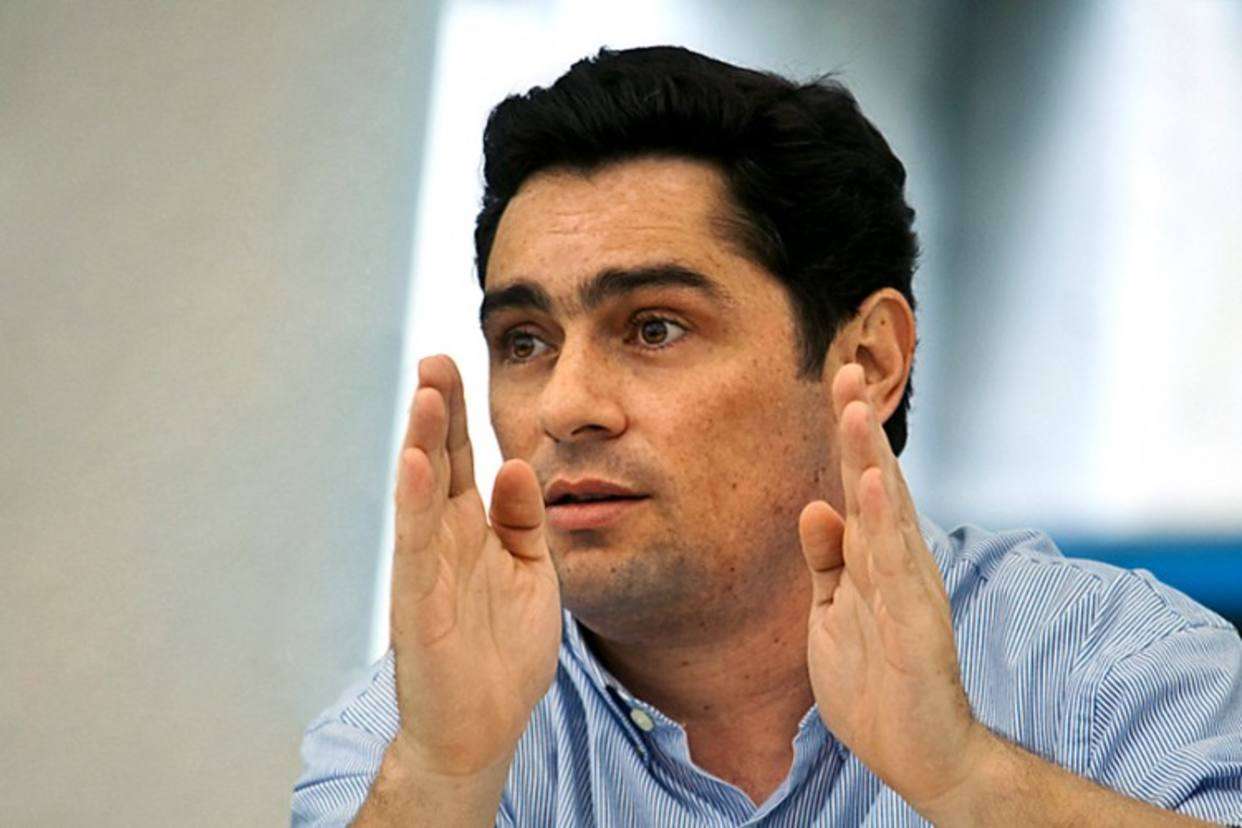
\includegraphics[width=300px]{EN_273307.jpg}%
\newline%
%
Carlos Vecchio, el embajador de Venezuela ante Estados Unidos, reiteró este lunes que si el oficialismo intenta detener al presidente de la Asamblea Nacional y presidente interino de Venezuela, Juan Guaidó, esto aceleraría la salida de Maduro del poder.%
\newline%
%
Mediante Twitter, el diplomático recordó que en enero de este año Maduro ordenó detener al líder opositor.%
\newline%
%
"Sabemos el efecto que eso produjo", escribió en la red social.%
\newline%
%
El embajador aseguró que la detención de Guadió significaría el error más grande que pudieran cometer~los oficialistas.%
\newline%
%
\end{document}